\usetikzlibrary{arrows.meta}
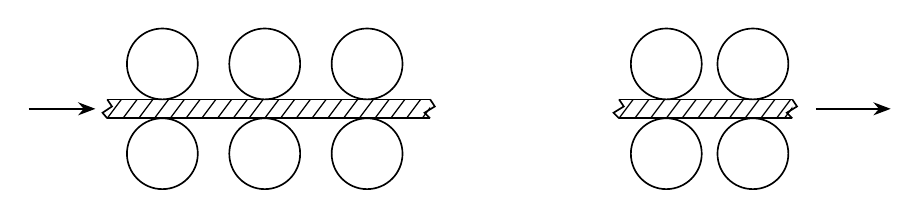
\begin{tikzpicture}[x=1cm,y=1cm,line width=.6pt,font=\normalsize]
% left hatched strip
\begin{scope}
\clip (-0.6,-0.12) rectangle (3.5,0.12);
\foreach \x in {-0.8,-0.6,-0.4,-0.2,0,0.2,0.4,0.6,0.8,1.0,1.2,1.4,1.6,1.8,2.0,2.2,2.4,2.6,2.8,3.0,3.2,3.4} {
\draw[line width=.45pt] (\x,-0.12) -- (\x+0.18,0.12);
}
\end{scope}
\draw (-.6,-.12)--(3.5,-.12);\draw (-.6,.12)--(3.5,.12);
\draw (-.6,-.12)--(-.66,-.05)--(-.54,.03)--(-.6,.12);
\draw (3.5,-.12)--(3.43,-.05)--(3.56,.03)--(3.5,.12);
% right hatched strip
\begin{scope}
\clip (5.9,-0.12) rectangle (8.1,0.12);
\foreach \x in {5.7,5.9,6.1,6.3,6.5,6.7,6.9,7.1,7.3,7.5,7.7,7.9,8.0} {
\draw[line width=.45pt] (\x,-0.12) -- (\x+0.18,0.12);
}
\end{scope}
\draw (5.9,-.12)--(8.1,-.12);\draw (5.9,.12)--(8.1,.12);
\draw (5.9,-.12)--(5.83,-.05)--(5.96,.03)--(5.9,.12);
\draw (8.1,-.12)--(8.03,-.05)--(8.16,.03)--(8.1,.12);
% rollers: true circles tangent to strip faces
\draw (0.1,0.57) circle[radius=0.45];
\draw (0.1,-0.57) circle[radius=0.45];
\draw (1.4,0.57) circle[radius=0.45];
\draw (1.4,-0.57) circle[radius=0.45];
\draw (2.7,0.57) circle[radius=0.45];
\draw (2.7,-0.57) circle[radius=0.45];
\draw (6.5,0.57) circle[radius=0.45];
\draw (6.5,-0.57) circle[radius=0.45];
\draw (7.6,0.57) circle[radius=0.45];
\draw (7.6,-0.57) circle[radius=0.45];
% entry / exit arrows
\draw[-{Stealth[length=2.2mm]}] (-1.6,0) -- (-0.75,0);
\draw[-{Stealth[length=2.2mm]}] (8.4,0) -- (9.35,0);
\end{tikzpicture}
